%!TEX TS-program=xelatex
%!TEX encoding=utf8
\documentclass[xelatex,hyperref=xdvipdfmx,11pt]{beamer}

%%%% XeLaTeX-Support %%%%
% \usepackage{xltxtra}

%%%% Encoding %%%%
\usepackage[utf8]{inputenc}
\usepackage[T1]{fontenc}

%%%% Pakete, die nie fehlen dürfen %%%%
\usepackage{graphicx}
\usepackage{xcolor}
\usepackage[german=swiss]{csquotes}

\usepackage{tabularx}
\usepackage{booktabs}

% \usepackage{amsmath}
% \usepackage{breqn}
% \usepackage{unicode-math}

%%%% Sprache %%%%
% \usepackage{polyglossia}
% \setmainlanguage[spelling=new]{german}

%%%% Schriften %%%%
% \setmainfont[Path = /home/christian/.fonts/,UprightFont = *Regular.otf,ItalicFont = *Italic.otf,BoldFont = *Bold.otf,BoldItalicFont = *BoldItalic.otf,Mapping=tex-text,Numbers={Uppercase,Proportional}]{CallunaSans}

% \setsansfont[Path = /home/christian/.fonts/,UprightFont = *Regular.otf,ItalicFont = *Italic.otf,BoldFont = *Bold.otf,BoldItalicFont = *BoldItalic.otf,Mapping=tex-text,Numbers={Uppercase,Proportional}]{CallunaSans}

% \setmonofont[Scale=MatchLowercase]{Inconsolata}


%%%% Formatierung %%%%
\useoutertheme{infolines}
\usecolortheme{whale}
\usecolortheme{dolphin}
\setbeamercolor*{titlelike}{parent=structure}
\usefonttheme[onlysmall]{structurebold}
\beamertemplatenavigationsymbolsempty
\setbeamercovered{transparent}
\providecommand{\alert}[1]{\textbf{#1}}
\setbeamertemplate{section in toc}{\leavevmode\leftskip=1ex\inserttocsectionnumber.\leavevmode\kern1ex\inserttocsection\par\kern5pt}
\setbeamertemplate{subsection in toc}{\leavevmode\leftskip=5ex{\usebeamercolor[fg]{structure}•}\protect\protect\hspace{1.5ex}\inserttocsubsection\par\kern2pt}
\setbeamertemplate{itemize item}{•}


%%%% Titelinfo %%%%
\title[\LaTeX für Politikwissenschafter – Teil 1]{\LaTeX{} für Politikwissenschafter}
\subtitle{Teil 1: Einführung und Installation}
\author[Christian und Nicolas]{Christian Müller \and Nicolas Zahn}
\institute[polito]{polito – Fachverein Politikwissenschaft}
\date{TBA}


%%%%%%%%%%%%%%%%%%%
% Beginn Dokument %
%%%%%%%%%%%%%%%%%%%

\begin{document}

\maketitle


\frame{
\frametitle{Wieso \LaTeX?}

\hbox to .6\textwidth{%
\Large%
\kern 2cm
\vbox{%
\hbox{\LaTeX{} makes the easy things harder,}%
\hbox{the harder things easier,}%
\hbox{and the impossible things possible.}%
}%
}

\vspace{.5cm}

{\makebox{}\hspace{.55\textwidth}— frei nach Richard D. Morey}\par

}

\frame{
\frametitle{Was kann man mit \LaTeX{} machen?}

\begin{itemize}
    \item Gut aussehende Dokumente produzieren, ohne viel Zeit für 
	Formatierung zu verbrauchen.
    \item Automatisch (!) in allen gängien Stilen Zitieren und 
	Bibliographieren.
    \item Verzeichnisse (Inhaltsverzeichnis, Tabellen- und/oder
	Abbildungsverzeichnis, Stichwortverzeichnis, usw. …) werden 
	automatisch erstellt und sind immer korrekt (!).
    \item Alle Dokumente als \emph{plaintext}-Format speichern. {\small 
	(erleichtert u.\thinspace a. die Zusammenarbeit mit Mitautoren und 
	ermöglich die Verwendung von Versionskontrollsystemen (git, …))}
\end{itemize}



}

\frame{
\frametitle{Aufbau der Einführung}

\begin{enumerate}
  \item Einführung und Installation (heute, 18.10.)
    \begin{itemize}
      \item Einführung in WYSIWYM
      \item \textbf{Installation Distribution und Editor (auf dem
	  mitgebrachten Computer)}
    \end{itemize}
  \item Arbeiten schreiben mit \LaTeX{} (25.10.)
    \begin{itemize}
      \item TBD % TODO
    \end{itemize}
  \item Präsentationsfolien mit \LaTeX{} (1.11.)
    \begin{itemize}
      \item Einführung ins \texttt{beamer}-Paket
    \end{itemize}
\end{enumerate}

}


\frame{
\frametitle{Übersicht heute (Einführung und Installation)}

\tableofcontents

}




\section{\LaTeX{} Grundlagen}
\label{sec:grundlagen}


\subsection{Distributionen und Editoren}
\label{sec:install}

\frame{

% TODO Einführung der Konzepte Editor/Distribution

}


\subsection{Begriffe}
\label{sec:begriffe}

\begin{frame}
\frametitle{\TeX und \LaTeX}

\begin{itemize}
\item \TeX{} wurde von Donald E. Knuth als Mathematiksatzprogramm entwickelt
\item die erste Version wurde 1982 veröffentlicht
\item \LaTeX{} ist eine Sammlung von Makros für \TeX
\item \LaTeX{} wurde von Leslie Lamport (La(mport)\TeX ) enwickelt und wird zurzeit
     von Frank Mittelbach betreut
   \item die derzeitige \LaTeX -Version ist LaTeX2$_{\epsilon}$
\item \LaTeX 3 ist in Entwicklung
\item sonstige Engines: teTeX, Xe(La)\TeX{}, eTeX
\end{itemize}
\end{frame}


\subsection{WYSIWYG und WYSIWYM}
\label{sec:wysiwym}

\frame[label={wysiwyg}]{
\frametitle{WYSIWYG v. WYSIWYM}

\begin{block}{\enquote{What you see is what you \textbf{get}} (WYSIWYG)\hfill\hyperlink{anhang:beispiel-libreoffice}{\beamergotobutton{Beispiel LibreOffice}}}<1->
    \begin{itemize}
	\item Programme: Word, LibreOffice, InDesign, …
	\item Man sieht und editiert das Enddokument 1:1 auf dem
	  Bildschirm 
    \end{itemize}
\end{block}


\begin{block}{\enquote{What you see is what you \textbf{mean}} (WYSIWYM) \hfill\hyperlink{anhang:beispiel-latex-1}{\beamergotobutton{Beispiel \LaTeX{}}}}<2->
  \begin{itemize}
    \item Markup-Languages: (La)TeX, HTML, DocBook, …
    \item Zwei Dokumente: Quellcode (Source) und (kompiliertes)
      Enddokument
    \item Editiert wird der Quellcode …
    \item … dieser wird dann kompiliert …
    \item … das ergibt das Enddokument
  \end{itemize}
\end{block}

}



\frame{
\frametitle{Source-Code und Kompilation}

% TODO Einführung Konzepte Sourcecode und Kompilation

}


\frame{
\frametitle{Vor- und Nachteile von WYSIWYM}

\begin{columns}

\begin{column}{.5\textwidth}
  \begin{block}{Vorteile}
    \begin{itemize}
      \item … % TODO Vorteile WYSIWYM
    \end{itemize}
  \end{block}
\end{column}

\begin{column}{.5\textwidth}
  \begin{block}{Vorteile}
    \begin{itemize}
      \item … % TODO Nachteile WYSIWYM
    \end{itemize}
  \end{block}
\end{column}

\end{columns}

}



\section{Erste Schritt}
\label{sec:erste-schritte}

% TODO Einführungsdokument erstellen. 
% Inhalt:
% - Aufbaukommandos (section etc.)
% - Schriftumschaltung (\bfseries etc.)
% - Textausrichtung (\centering etc.)
% - Math-Mode

% TODO Folien zur Erklärung des Einführungsdokuments.


\section*{Literatur}
\label{sec:literatur}

\begin{frame}
\frametitle{Literatur}

\setbeamertemplate{bibliography item}[article] 
\scriptsize
\begin{thebibliography}{}

\bibitem{lshort} Tobias Oetiker, Hubert Partl, Irene Hyna und Elisabeth Schlegl
\newblock The Not So Short Introduction to LaTeX $2_{\epsilon}$
\newblock Online im Internet. URL: \url{http://www.ctan.org/get/info/lshort}.

\setbeamertemplate{bibliography item}[book]

\bibitem{companion}  Frank Mittelbach und Michel Goossens mit Hohannes Braams, David Carlisle und Chris Rowley (2006)
\newblock The \LaTeX Companion
\newblock 2. Auflage. Boston: Addison-Wesley.

\end{thebibliography}
\end{frame}


\section*{Anhang}
\label{sec:anhang}

\frame[label={anhang:beispiel-libreoffice}]{
\frametitle{Beispiel WYSIWY\textbf{G}: LibreOffice} % Microsoft
% Word\char"000AE}

\centering

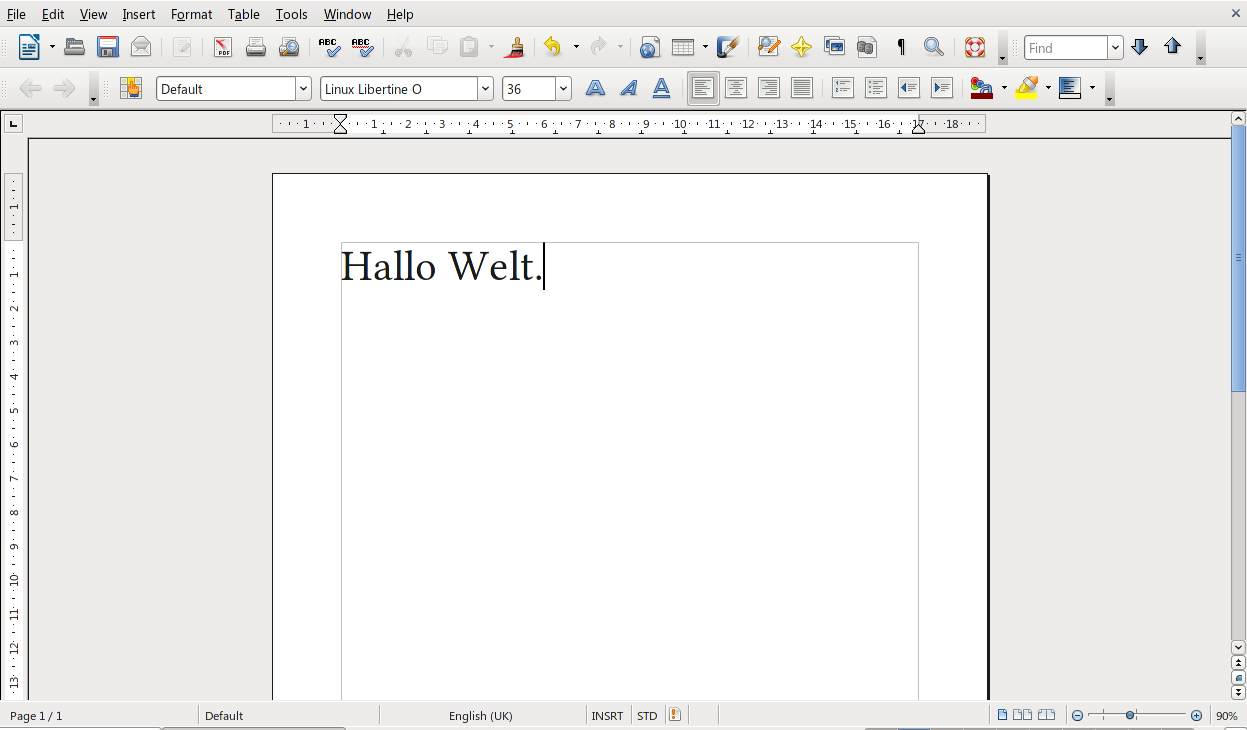
\includegraphics[width=0.9\textwidth]{wysiwyg-libreoffice.png}

\vfill

\hfill\hyperlink{wysiwyg<1>}{\beamerreturnbutton{Zurück}} 
}

\begin{frame}[fragile,label={anhang:beispiel-latex-2}]
\frametitle{Beispiel WYSIWY\textbf{M}: \LaTeX{} }

\begin{verbatim}

\frame{
\frametitle{Das ist eine einfache Beispielseite}

Hallo Welt

}

\end{verbatim}

\end{frame}


\frame[label={anhang:beispiel-latex-1}]{
\frametitle{Das ist eine einfache Beispielseite}

\vfill

Hallo Welt

\vfill

\hfill\hyperlink{wysiwyg<2>}{\beamerreturnbutton{Zurück}} 
}




\end{document}

